% !TEX root=../pldi2019.tex



\section{Language}
\label{sec:language}

\fixme{Introduce \TOPHAT here}

\subsection{Expressions}

\label{sub:expressions}
The host language is a simply typed lambda calculus, extended with some basic types and \ML-style references.
The grammar in \cref{fig:language-grammar} defines the syntax of the host language.
It has abstractions, applications, variables, and constants for booleans, integers and strings.
The symbol $\star$ stands for binary operators.
For the result of parallel tasks we need pairs.
Conditionals come in handy for defining guards.
References will be used to implement shared editors.
Our treatment of references closely follows the one by \citet{books/Pierce02TAPL}.
Creating a reference using the keyword $\Ref$ yields a location $l$.
Locations are not intended to be directly manipulated by the programmer.
The symbols ! and $:=$ stand for dereferencing and assignment.
The unit value will be used as the result of assignments.

\begin{figure}[h]
  \small
  \usemacro{G-Language-Compact}
  \caption{Language grammar} \label{fig:language-grammar}
\end{figure}

\label{sub:notation}
We use double quotation marks to denote strings.
Integers are denoted by their decimal representation, and booleans are written $\True$ and $\False$.
We freely make use of the logic operators $\Not$, $\land$, and $\lor$, arithmetic operators $+$, $-$, $\times$, and the string append operator $\pp$.
Furthermore, we use standard comparison operations $<$, $\le$, $\equiv$, $\not\equiv$, $\ge$, and $>$.
The symbol $\star$ stands for any of those.

\label{sub:abbreviations}
The notation $e_1; e_2$ is an abbreviation for $(\lambda x:\Unit.\ e_2)\ e_1$, where $x$ is a fresh variable.
The notation $\Let x:\tau = e_1 \In e_2$ is an abbreviation for $(\lambda x:\tau.\ e_2)\ e_1$.

\label{sub:pretasks}
The grammar in \cref{fig:task-grammar} specifies the syntactic category of \emph{pretasks}.
Pretasks are tasks that have unevaluated subexpressions.
Pretasks are discussed in more detail in the following sections.
We use open symbols ($\Edit, \Enter, \Next, \Xor$) for tasks that require user input, and closed symbols ($\Update, \Then, \Or$) for tasks that can be evaluated without user input.

\begin{figure}[h]
  \small
  \usemacro{G-Pretasks-Compact}
  \caption{Task grammar} \label{fig:task-grammar}
\end{figure}



\paragraph{Typing}
\label{sub:typing}

% Typing of our expressions $e$ is as to be expected.
% and won't be given in this document.
\Cref{fig:type-grammar} shows the grammar of types used by \TOPHAT.
It has functions, pairs, basic types, unit, references, and tasks.

\begin{figure}[h]
  \small
  \usemacro{G-Types-Compact}
  \caption{Type grammar} \label{fig:type-grammar}
\end{figure}

Typing rules are of the form $\RelationT$, which should be read as \enquote{in environment $\Gamma$ and store typing $\Sigma$, expression $e$ has type $\tau$}.
Typing rules for expressions in the host language are presented in the appendix.
The typing rules for pretasks are given in \cref{fig:typing-rules}.

\begin{figure}[h]
  \small
  \begin{mathpar}
    \boxed{\RelationT} \\
    \userule{T-Edit} \quad
    \userule{T-Enter} \quad
    \userule{T-Update} \\
    \userule{T-Then} \quad
    \userule{T-Next} \\
    \userule{T-Fail} \quad
    \userule{T-And} \\
    \userule{T-Or} \quad
    \userule{T-Xor}
  \end{mathpar}
  \caption{Typing rules} \label{fig:typing-rules}
\end{figure}



\subsection{Editors}

Programs in \TOPHAT model interactive workflows.
Interaction means communication with end users.
End users should be able to enter information into the system, change it, clear it, reenter it, and so on.
To do this, we introduce the concept of editors.

Editors are typed containers that either hold a value or are empty.
Editors that have a value can be \emph{changed} or \emph{emptied}.
Empty editors can be \emph{filled}.
This is depicted as a state diagram in \cref{fig:editor-state} below.

\begin{figure}[h]
  \centering
  \includegraphics[width=\columnwidth,page=3]{figures/drawings-crop.pdf}
  \caption{
    Possible states of an editor and its transitions.
    Shared editors cannot be cleared.
  }
  \label{fig:editor-state}
\end{figure}

Editors stand for various forms of input and output, for example widgets in a \GUI, form fields on a webpage, sensors, or network connections.

Consider the editor for a person's age from \cref{exm:flight-booking}.
Users can change the value until they are satisfied with it.
Editors are meant capture this constantly changing nature of user input.

The user interface of an editor depends on its type.
This could be an input field for strings, a toggle switch for booleans, or even a map with a pin for locations.
It could also be a parser that tries to parse a line of text to match the type of the editor.


\paragraph{Valued and unvalued editors $(\Edit e, \Enter \tau)$}

Editors that hold an expression $e : \tau$ have type $\Task \tau$.
Empty editors are annotated with a type in order to ensure type safety.
Without that it would be possible to change the type of an editor, by clearing it and filling it with a value of different type.

\paragraph{Shared editors $(\Update e)$}

Shared editors watch references, lifting their value into the task domain.
If $e$ is a reference $\Reference \tau$, then $\Update e$ is of type $\Task \tau$.
Shared editors cannot be cleared, only changed.

Changes to a shared editor are immediately visible to all shared editors watching the same reference.
Imagine two users, Marco and Christopher, both watching shared editors of the same coordinate.
The editors are visualized as a map with a pin.
When Marco moves his pin, he updates the value of the shared editor, thereby changing the value of the reference.
This change is immediately reflected on Christopher's screen: The pin changes its position on his map.
This way Marco and Christopher can work together to edit the same information.

\label{sub:time}
Two other important use cases for shared editors are sensors and time.
Sensors can be represented as external entities that periodically update a shared editor with their current sensor value.
Similarly, the current time can be stored in a shared editor which is periodically updated by a clock.
The actual sensor and the clock are not modelled in \TOPHAT.
We assume that they exist as external users that send update events to the system.
This allows programmers to write tasks that react to sensor values or timeouts.


\subsection{Steps}

Editors represent atomic units of work.
In this section we look at ways to combine smaller tasks into bigger ones.
Combining tasks can be done in two ways, sequential and parallel.
Parallel composition comes in two variants: combining two tasks (\emph{and}-parallel) and choosing between two tasks (\emph{or}-parallel).
We study sequential composition first, and after that combining and choosing.


\paragraph{Internal and external step $(t \Then e, t \Next e)$}
\label{sub:steps}

Sequential composition has a task $t$ on the left hand side and a continuation $e$ on the right.
The accompanying typing rules are \refrule{T-Then} and \refrule{T-Next}.
According to these rules, the left hand side must be a task $t : \Task \tau_1$, and the right hand side $e : \tau_1 \to \Task \tau_2$ must be a function that, given the task value of $t$, calculates the task with which to continue.

Steps are guarded, which means that the step combinators can only proceed when the following conditions are met.
The left hand side must have a value, only then can the right hand side calculate the successor task.
The successor task must not be $\Fail$, introduced below.
The internal step can proceed immediately when these conditions are met.
The external step must additionally receive a continue event $\Continue$.


\begin{example}[Conditional stepping]
\label{exm:conditions}

Consider the following program.
\begin{TASK}
  enter Int >>= \n. if n == 42 then edit "Good" else edit "Bad"
\end{TASK}
Initially the step is guarded because the editor doesn't have a value.
When the user enters an integer, the program continues immediately with either \TS|edit "Good"| or \TS|edit "Bad"|, depending on the input.

\end{example}




\paragraph{Fail $(\Fail)$}
\label{sub:fail}

Fail is a task that never has a value and never accepts input.
The typing rule \refrule{T-Fail} states that it has type $\Task \tau$ for any type $\tau$.
Programmers can use $\Fail$ to tell steps that no sensible successor task can be determined.

\begin{example}[Guarded stepping]

Consider the following program.
\begin{TASK}
  enter Int >>= \n. if n == 42 then edit "Good" else fail
\end{TASK}
The user is asked to enter an integer.
As long as the right hand side of $\Then$ evaluates to $\Fail$, the step cannot proceed, and the user can keep editing the integer.
As soon as the value of the left hand side is $42$, the right hand side evaluates to something other than $\Fail$, and the step proceeds to \TS{edit "Good"}.

\end{example}



\begin{example}[Waiting]\label{exm:wait}

\lstset{emph={delay,start,now}}
With the language constructs seen so far it is possible to create a task that delays execution for a specified delay of time.
To do this,
we make use of a shared editor holding the current time (see \cref{sub:time}),
and a guarded internal step.
\begin{TASK}
  let wait : Int -> Task Unit = \delay : Int.
    update time >>= \start : Int.
    update time >>= \now : Int.
      if now >= start + delay then edit <<>> else fail
\end{TASK}
The first step is immediately taken, resulting in \TS{start} to be the time at the moment \TS{wait} is executed.
The second step is guarded until the current time is greater or equal to the start time plus the requested delay.

\end{example}



\subsection{Parallel}

A common pattern in workflow design is splitting up work into multiple tasks that can be executed simultaneously.
In \TOPHAT, all parallel branches can progress independently, driven by input events.
This requires input events to be tagged in order to reach the intended task.

There are two ways to proceed after a parallel composition.
One way is to wait for all tasks to produce results and combine those,
the other to pick the first available result.
Both ways introduce explicit forks and implicit joins in \TOPHAT.


\paragraph{Combination $(e_1 \And e_2)$}

A combination of two tasks is a parallel \emph{and}.
It has a value only if both branches have a value.
This is reflected in the typing rule \refrule{T-And},
It shows that if the first task has type $\tau_1$,
and the second has type $\tau_2$,
their combination has the pair type $\tau_1 \times \tau_2$.



\begin{example}[Combining]

The task
\begin{TASK}
  enter Int <&> edit " Batman" >>= \<<n, s>>. edit (replicate n "Na" ++ s)
\end{TASK}
can only step when both editors have values.
When it steps, the continuation uses the pair of integer and string to calculate the result.

\end{example}


\paragraph{Internal and external choice $(e_1 \Or e_2, e_1 \Xor e_2)$}

Where combinations wait for both tasks to produce results,
internal choices pick one branch as soon as it has a result.
Its typing rule \refrule{T-Or} therefore dictates that both branches should have the same type $\Task \tau$.
E.g. $\Edit 37 \Or \Enter \Int$ will result in $\Edit 37$ directly,
because $\Enter \Int$ does not contain a value.
To make \TOPHAT deterministic,
we always prefer the first task over the second.

As with combinations, users can work on both tasks of an internal choice ($\Or$) simultaneously.
However, this does not hold for external choice ($\Xor$).
External choices await user input to pick the left or right branch before continuing with that task.
This means one cannot work on both branches of an external choice before picking one or the other.



\begin{example}[Delay]

\lstset{emph={proceed}}

To illustrate the usage of internal and external choices,
we will create an example that will ask users explicitly to proceed with a task or to cancel.
When users do not make a choice within a given amount of time,
we will automatically proceed.
To do this,
we will make use of the \TS{wait}-task from \cref{exm:wait}.
\begin{TASK}
  let cancel : Task Unit = edit <<>> in
  let delay : Int -> Task Unit -> Task Unit =
    \n : Int. \proceed : Task Unit.
    (proceed <?> cancel) <|> (wait n >>= \u : Unit. proceed)
\end{TASK}
Note this task is higher-order:
it is a task which takes another task as a parameter.

\end{example}

% \subsection{Appointment}
%
% \fixme{write this subsection}

% It is essential for a workflow system to support multiple collaborators working
% together. Adding this funcitonaltiy to the \TOPHAT calculus is very
% straightforward. We identify users by means of a name $u$ which we can then use
% to label appointed tasks. The sole purpose of this labelling is to be able to
% tell which inputs are expected from what users. Other than that, it has no
% influence on the semantics. For space reasons, we have have excluded multi-user
% support from this paper.
%
% Mss moeten we het schrijven vanuit het oogpunt van labeling: je kunt labels
% toevoegen aan knoppen, als uitleg bij taken en om gebruikers toe te kennen aan
% taken. Vervolgens zou je iets met die gebruikers kunnen doen: alleen taken voor
% hun weergeven in de UI, alleen inputs voor hun genereren met I etc. Past dat?

\subsection{Annotations}

Lastly, pretasks can be annotated with additional information.
This information can then be used to modify the user interface, or for analysis
purposes like resource analysis, or automatic end-user feedback. In the case of
user interface, one could think of labelling information for buttons,
or with descriptions of tasks.
We have implemented annotating pretasks with user information to support
multiple users working together, this has been ommitted from the semantics
in this paper for space reasons. The annotated user information is used to build
an interface specific to the user, only displaying actions that she can take.

Resouce analysis and automatic end-user feedback for \TOPHAT is left for future
work.


% For now, we only concentrate on appointing tasks to users,
% which is common in workflow modelling.
%
%
%
% \paragraph{Appoint $(u \At e)$}
%
% Users are identified by a name $u$ which is a string.
% They can be appointed tasks by means of the $\At$ combinator.
% The sole purpose of this labelling is to be able to tell users which inputs are expected of them.
% In \cref{sec:handling}, a function is described to calculate which users can take what actions.
% Other than this function, the appointment of tasks has no influence on the semantics.
% All semantic rules in \cref{sec:semantics} simply continue with their operations as if the label was not there.
% \todo{we still have to fix the type of $\Inputs$ and state the type of $u$}
